\chapter{RL basics}
At first we have to define an environment where agent can operate. Environment can be described as Markov decision process, where $S_t \in \mathcal{S}$ is state from set of possible states $\mathcal{S}$ in which is the environment located in time $t$. Agent can observe environment's state and take action accordingly. Action is a transition between states. Every action $A_t \in \mathcal{A}$ moves the environment from $S_t$ to $S_{t+1}$. Environment evaluates every action and return appropriate reward $R_t$. In RL is set $\mathcal{A}$ often called action space and set $\mathcal{S}$ observation space. Agent's main goal is to maximise reward.

\begin{figure}[!h]
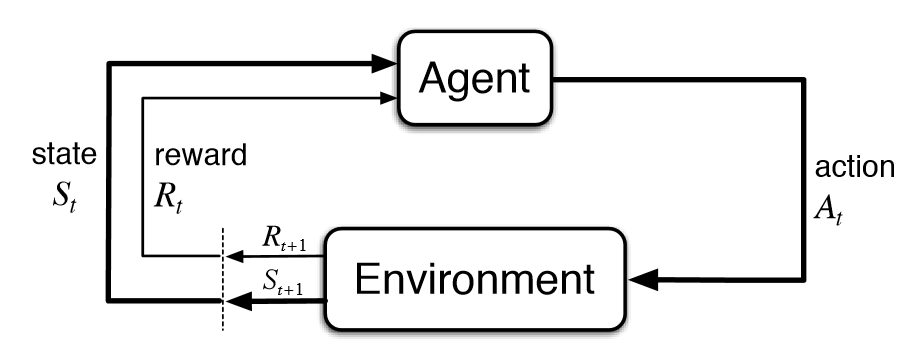
\includegraphics[scale=0.3]{images/RL-concept.png}
\caption{RL concept}
\end{figure}

Major issue is that maximising immediate reward often isn't good approach to maximise overall reward. This greedy policy can take us into very disadvantageous states. Thus agent must take in account future states and rewards. In past agents used to contain big tables which stored information about quality of every action in every state. That is possible in environments with small action and observation spaces, but very memory consuming for larger environments and even impossible for continuous action or observation space. Therefore modern methods use neural networks as function approximators.

\section{Temporal difference learning}
Temporal difference (TD) learning is combining ideas of Monte Carlo methods and dynamic programming. It is able to learn directly from experience obtained by interactions with environment without any knowledge about environment. TD learning is done by following assignment in each timestamp [Sutton]
\begin{equation}
V(S_t) \gets V(S_t) + \alpha [R_{t+1} + \gamma V(S_{t+1}) - V(S_t)]
\end{equation}
where $V$ is so called state value, which tells us how good is being in particular state with current policy. $\alpha \in \mathbb{R}^+$ is step size and $\gamma \in (0, 1)$ is discount factor.

\section{Q-learning}
Q-learning is type of TD learning developed by Watkins [1989]. The state value $V$ from previous section is replaced by $Q$ value, which refers to quality of action in particular state instead of quality of state itself. When we rewrite TD learning (1.1) to Q-learning we get:
\begin{equation}
Q(S_t, A_t) \gets Q(S_t, A_t) + \alpha [R_{t+1} + \gamma max_{A_{t+1}} Q(S_{t+1}, A_{t+1}) - Q(S_t, A_t)].
\end{equation}
Our policy here is to take action with maximal $Q$ value. That is called greedy policy. Obvious drawback of greedy policy is that we won't explore whole environment properly, because in some states we would always take same action with highest $Q$ value. Solution to this problem is sometimes take random action to explore the environment. This policy is often referred as $\epsilon$-greedy policy.

\begin{algorithm}
\caption{$\epsilon$-greedy policy}\label{euclid}
\begin{algorithmic}[1]
\Procedure{ChooseAction}{}
\State $\epsilon \gets \epsilon \cdot \epsilon_d$
\If {$\epsilon >$ random $\in (0,1)$}
\State action $\gets$ random $\in \mathcal{A}$
\Else 
\State action $\gets$ $argmax_{A_t} Q(S_t, A_t)$
\EndIf
\State \Return action
\EndProcedure
\end{algorithmic}
\end{algorithm}

It is common to set $\epsilon = 1$ at the beginning of the training and decay rate $\epsilon_d$ close to one. This policy assumes that at first you need to explore environment and then exploit agent's experience.

\chapter{Deep neural networks in RL}
As we stated in previous chapter, tabular methods are very inefficient when it comes to large environments. Here comes in play deep neural networks which can replace tables. Deep Q networks (DQN) proposed by Google's Deepmind [2015] outperformed all previous RL algorithms in playing Atari games. With neural networks grew also popularity of policy gradient methods [Sutton], where neural network outputs specific action instead of Q values.

\section{DQN}
Neural network takes current state as input and outputs Q value for each possible action. Network is trained using gradient descent. As loss function $L$ is commonly used mean squared error between currently predicted Q value and target value $Y$
\begin{equation}
Y = R_{t+1} + \gamma max_{A_{t+1}}Q(S_{t+1}, A_{t+1};\theta)
\end{equation}
\begin{equation}
L = \frac{1}{2}[Y - Q(S_t, A_t;\theta)]^2
\end{equation}
where $\theta$ is set of weights of our function estimator (neural network). Unfortunately this simple DQN agent suffers from lack of sample efficiency and does not converge well. There is a lot of techniques which can help DQNs to achieve good results.

\subsection{Target network}
Target network is technique proposed by Mnih[Citace] to improve convergence of DQN learning. It uses two neural nets instead of one. We train first - training network on batch of data, but we use second - target network for predictions during training. When is training on batch completed, we update target network.
\begin{equation}
\theta^- = \tau \theta + (1-\tau)\theta^-
\end{equation}
where $\theta^-$ is set of trainable weights of target network, $\theta$ indicates online network weights and $\tau << 1$ is constant.
Our target value $T$ is now calculated using target network:
\begin{equation}
Y = R_{t+1} + \gamma max_{A_{t+1}}Q(S_{t+1}, A_{t+1};\theta^-)
\end{equation}
Target network stabilize training since predicting network isn't changing after every training step.

\subsection{Prioritized experience replay}
Experience replay is biologically inspired mechanism proposed by [Schaul-citace] which stores all experiences (specifically: $S_t$, $A_t$, $R_{t+1}$, $S_{t+1}$) into buffer and assign priority to every experience. Main idea is that experiences with high TD error should have higher priority. For TD error applies:
\begin{equation}
TD_{error} = |Y - Q(S_t, A_t;\theta)|.
\end{equation} 
Further is necessary to calculate priority $p$ from TD error:
\begin{equation}
p = (TD_{error} + \beta)^\alpha
\end{equation}
where $\alpha$ tells us how much we would like to prefer experience with higher priority and $\beta << 1$ is a constant which helps us to avoid priorities very close to zero. Whereas greedy selection would abandon experiences with low priority, better approach is to choose experience $i \in \mathcal{I}$ with probability:
\begin{equation}
P(i) = \frac{p_i}{\sum_{\forall j \in \mathcal{I}} p_j}
\end{equation}
where $\mathcal{I}$ is set of all experiences in buffer. Now we can sample batch of experiences for training using this probability. It removes correlation in the observation sequence and improves sample efficiency of DQN. It is possible to store all experiences in buffer sorted by priority, but much more efficient implementation is a sum tree.

\subsection{Double Q-learning}
Classic Q-learning algorithm tends to overestimate actions under certain conditions. Hasselt et al [citace] propose idea of Double Q-learning which decompose the max operation into action selection and action evaluation. Target value is then computed by following equation.
\begin{equation}
Y = R_{t+1} + \gamma Q(S_{t+1}, argmax_{A_{t+1}}Q(S_{t+1}, A_{t+1};\theta);\theta^-).
\end{equation}
Double DQN outperforms DQN in terms of value accuracy and in terms of policy quality.